\documentclass[12pt]{article}
\usepackage[danish]{babel}
\usepackage{amsfonts, amssymb, mathtools, amsthm, amsmath}
\usepackage{graphicx, pgfplots}
\usepackage{url}
\usepackage[dvipsnames]{xcolor}
\usepackage{sagetex}
\usepackage{lastpage}

%loaded last
\usepackage[hidelinks]{hyperref}

\usepackage{siunitx}
  \sisetup{exponent-product = \cdot,
    output-decimal-marker = {,}}

%Giles Castelles incfig
\usepackage{import}
\usepackage{xifthen}
\usepackage{pdfpages}
\usepackage{transparent}

\newcommand{\incfig}[2][1]{%
  \def\svgwidth{#1\columnwidth}
  \import{../figures/}{#2.pdf_tex}
}

\setlength{\parindent}{0in}
\setlength{\oddsidemargin}{0in}
\setlength{\textwidth}{6.5in}
\setlength{\textheight}{8.8in}
\setlength{\topmargin}{0in}
\setlength{\headheight}{18pt}

\usepackage{fancyhdr}
\pagestyle{fancy}

\fancyhead{}
\fancyfoot{}
\fancyfoot[R]{\thepage}
\fancyhead[C]{\leftmark}

\pgfplotsset{compat=newest}

\pgfplotsset{every axis/.append style={
  axis x line=middle,    % put the x axis in the middle
  axis y line=middle,    % put the y axis in the middle
  axis line style={<->,color=black}, % arrows on the axis
}}

\usepackage{thmtools}
\usepackage{tcolorbox}
  \tcbuselibrary{skins, breakable}
  \tcbset{
    space to upper=1em,
    space to lower=1em,
  }

\theoremstyle{definition}

\newtcolorbox[auto counter]{definition}[1][]{%
  breakable,
  colframe=ForestGreen,  %frame color
  colback=ForestGreen!5, %background color
  colbacktitle=ForestGreen!25, %background color for title
  coltitle=ForestGreen!70!black,  %title color
  fonttitle=\bfseries\sffamily, %title font
  left=1em,              %space on left side in box,
  enhanced,              %more options
  frame hidden,          %hide frame
  borderline west={2pt}{0pt}{ForestGreen},  %display left line
  title=Definition \thetcbcounter: #1,
}

\newtcolorbox{greenline}{%
  breakable,
  colframe=ForestGreen,  %frame color
  colback=white,          %remove background color
  left=1em,              %space on left side in box
  enhanced,              %more options
  frame hidden,          %hide frame
  borderline west={2pt}{0pt}{ForestGreen},  %display left line
}

\newtcolorbox[auto counter, number within=section]{eks}[1][]{%
  brekable,
  colframe=NavyBlue,  %frame color
  colback=NavyBlue!5, %background color
  colbacktitle=NavyBlue!25,    %background color for title
  coltitle=NavyBlue!70!black,  %title color
  fonttitle=\bfseries\sffamily, %title font
  left=1em,            %space on left side in box,
  enhanced,            %more options
  frame hidden,        %hide frame
  borderline west={2pt}{0pt}{NavyBlue},  %display left line
  title=Eksempel \thetcbcounter: #1
}

\newtcolorbox{blueline}{%
  breakable,
  colframe=NavyBlue,     %frame color
  colback=white,         %remove background
  left=1em,              %space on left side in box,
  enhanced,              %more options
  frame hidden,          %hide frame
  borderline west={2pt}{0pt}{NavyBlue},  %display left line
}

\newtcolorbox{teo}[1][]{%
  breakable,
  colframe=RawSienna,  %frame color
  colback=RawSienna!5, %background color
  colbacktitle=RawSienna!25,    %background color for title
  coltitle=RawSienna!70!black,  %title color
  fonttitle=\bfseries\sffamily, %title font
  left=1em,              %space on left side in box,
  enhanced,              %more options
  frame hidden,          %hide frame
  borderline west={2pt}{0pt}{RawSienna},  %display left line
  title=Teori: #1,
}

\newtcolorbox[auto counter, number within=section]{sæt}[1][]{%
  breakable,
  colframe=RawSienna,  %frame color
  colback=RawSienna!5, %background color
  colbacktitle=RawSienna!25,    %background color for title
  coltitle=RawSienna!70!black,  %title color
  fonttitle=\bfseries\sffamily, %title font
  left=1em,              %space on left side in box,
  enhanced,              %more options
  frame hidden,          %hide frame
  borderline west={2pt}{0pt}{RawSienna},  %display left line
  title=Sætning \thetcbcounter: #1,
  before lower={\textbf{Bevis:}\par\vspace{0.5em}},
  colbacklower=RawSienna!25,
}

\newtcolorbox{redline}{%
  breakable,
  colframe=RawSienna,  %frame color
  colback=white,       %Remove background color
  left=1em,            %space on left side in box,
  enhanced,            %more options
  frame hidden,        %hide frame
  borderline west={2pt}{0pt}{RawSienna},  %display left line
}

\newtcolorbox{for}[1][]{%
  breakable,
  colframe=NavyBlue,  %frame color
  colback=NavyBlue!5, %background color
  colbacktitle=NavyBlue!25,    %background color for title
  coltitle=NavyBlue!70!black,  %title color
  fonttitle=\bfseries\sffamily, %title font
  left=1em,              %space on left side in box,
  enhanced,              %more options
  frame hidden,          %hide frame
  borderline west={2pt}{0pt}{NavyBlue},  %display left line
  title=Forklaring #1,
}

\newtcolorbox{bem}{%
  breakable,
  colframe=NavyBlue,  %frame color
  colback=NavyBlue!5, %background color
  colbacktitle=NavyBlue!25,    %background color for title
  coltitle=NavyBlue!70!black,  %title color
  fonttitle=\bfseries\sffamily, %title font
  left=1em,              %space on left side in box,
  enhanced,              %more options
  frame hidden,          %hide frame
  borderline west={2pt}{0pt}{NavyBlue},  %display left line
  title=Bemærkning:,
}

\makeatother
\def\@lecture{}%
\newcommand{\lecture}[3]{
  \ifthenelse{\isempty{#3}}{%
    \def\@lecture{Lecture #1}%
  }{%
    \def\@lecture{Lecture #1: #3}%
  }%
  \subsection*{\makebox[\textwidth][l]{\@lecture \hfill \normalfont\small\textsf{#2}}}
}

\makeatletter

\newcommand{\opgave}[1]{%
 \def\@opgave{#1}%
 \subsection*{Opgave #1}
}

\makeatother

%Format lim the same way in intext and in display
\let\svlim\lim\def\lim{\svlim\limits}

% horizontal rule
\newcommand\hr{
\noindent\rule[0.5ex]{\linewidth}{0.5pt}
}

\title{Afleveringsopgave uge 11}
\author{Noah Rahbek Bigum Hansen}
\date{12. November 2024}

\begin{document}

\maketitle

\section*{Opg. 6}
Betragt differentialligningen
\begin{equation} \label{eq:1}
  y' = \sin(y)
\end{equation}

\subsection*{1.}
Er differentialligningen (\ref{eq:1}) lineær?
\bigbreak
Idet differentialligningen ikke er en linearkombination af $y$ og $y$'s afledede er differentialligningen (\ref{eq:1}) ikke lineær.

\subsection*{2.}
Benyt Python til at løse differentialligningen \ref{eq:1} (numerisk) og plot din løsning med begyndelsesbetingelse $y(0) = 0$.
\bigbreak
Følgende prompt er givet til ChatGPT 4o: 

\begin{blueline}
  Write some python code that solves the differential equation y' = sin(y) for y(0) = 0 and plots the solution function
\end{blueline}

ChatGPT gav da følgende python-kode:
\begin{verbatim}
  import numpy as np
  import matplotlib.pyplot as plt
  from scipy.integrate import solve_ivp

  # Define the differential equation y' = sin(y)
  def dydt(t, y):
    return np.sin(y)

  # Initial condition y(0) = 0
  y0 = [0]

  # Time span for the solution
  t_span = (0, 10)
  t_eval = np.linspace(0, 10, 1000)

  # Solve the differential equation numerically
  solution = solve_ivp(dydt, t_span, y0, t_eval=t_eval)

  # Plot the numerical solution
  plt.plot(solution.t, solution.y[0], label="Numerical Solution")
  plt.xlabel("t")
  plt.ylabel("y(t)")
  plt.title("Solution of y' = sin(y) with y(0) = 0")
  plt.legend()
  plt.grid()
  plt.show()
\end{verbatim}

Hvilket giver følgende plot når koden køres
\begin{figure} [ht]
  \centering
  \caption{Resultat af python koden hvor løsningen til $y' = \sin(y); \quad y(0) = 0$ plottes}
  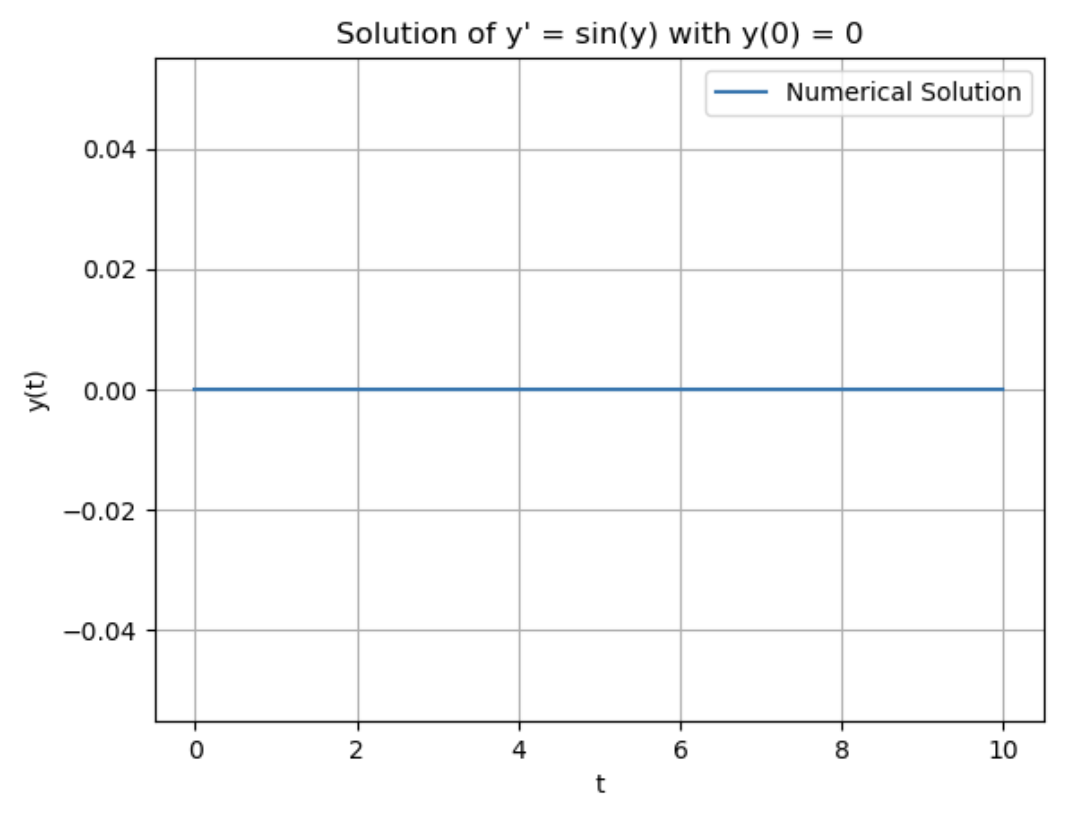
\includegraphics[width=0.8\linewidth]{../figures/A11_1.png}
  \label{fig:A11_1}
\end{figure}

Altså ses at løsningen til differentiallingen med den givne begyndelsesbetingelse er $y(t) = 0$, hvilket hurtigt kan ses er en korrekt løsning.


\subsection*{3.}
Benyt Python til at løse differentialligningen \ref{eq:1} (numerisk) og plot din løsning med begyndelsesbetingelse $y(0) = 1$. Sammenlign med resultatet fra punkt 2. Har startbetingelsen betydning for løsningen?
\bigbreak
Ved at ændre vores \textit{initial condition}, $y0$ i koden fra $[0]$ til $[1]$ og ellers opdaterer de andre steder hvor $y(0) = 0$ er brugt til $y(0) = 1$ kan vi omskrive Python-koden fra før til

\begin{verbatim}
  import numpy as np
  import matplotlib.pyplot as plt
  from scipy.integrate import solve_ivp

  # Define the differential equation y' = sin(y)
  def dydt(t, y):
    return np.sin(y)

  # Initial condition y(0) = 1
  y0 = [1]

  # Time span for the solution
  t_span = (0, 10)
  t_eval = np.linspace(0, 10, 1000)

  # Solve the differential equation numerically
  solution = solve_ivp(dydt, t_span, y0, t_eval=t_eval)

  # Plot the numerical solution
  plt.plot(solution.t, solution.y[0], label="Numerical Solution y(0) = 1")
  plt.xlabel("t")
  plt.ylabel("y(t)")
  plt.title("Solution of y' = sin(y) with y(0) = 1")
  plt.legend()
  plt.grid()
  plt.show()
\end{verbatim}

Når denne kode køres fås følgende plot

\newpage

\begin{figure} [ht]
  \centering
  \caption{Resultat af python koden hvor løsningen til $y' = \sin(y); \quad y(0) = 1$ plottes}
  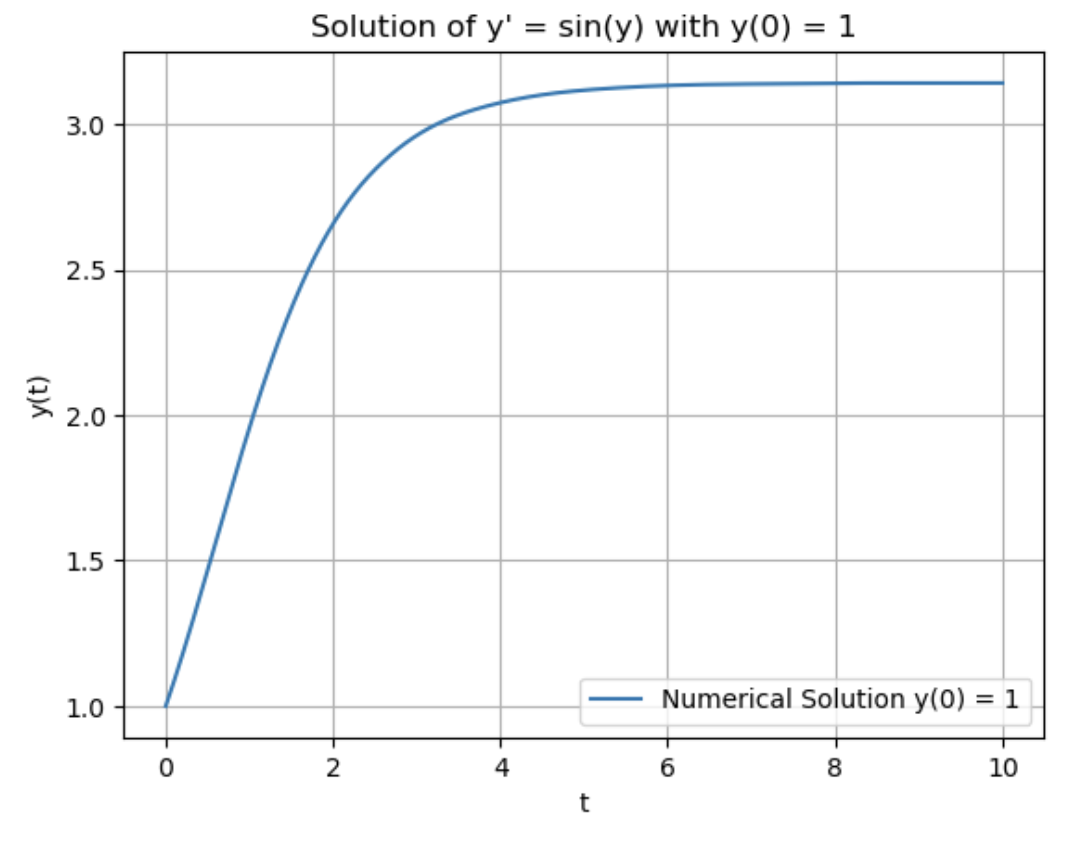
\includegraphics[width=0.8\linewidth]{../figures/A11_2.png}
  \label{fig:A11_2}
\end{figure}

Ved sammenligning af \autoref{fig:A11_1} og \autoref{fig:A11_2} kan ses at løsningen afhænger af bgyndelsesbetingelserne.


\section*{Opg. 7}
Lad $f(x,y)$ betegne funktionen
\[ 
f(x,y) = \sin(3y) e^{7x}
.\]

\subsection*{1.}
Udregn $\frac{\partial^2 f}{\partial x \partial y}$ ved hjælp af Python
\bigbreak
Følgende prompt er givet til ChatGPT 4o: 

\begin{blueline}
  Write some python code to calculate the pratial derivative with respect to x of the partial derivative with respect to y of $\sin(3y)e^{7x}$
\end{blueline}

ChatGPT gav da følgende python-kode:
\begin{verbatim}
  import sympy as sp

  # Define the variables
  x, y = sp.symbols('x y')

  # Define the function
  f = sp.sin(3*y) * sp.exp(7*x)

  # Calculate the partial derivative with respect to y
  partial_y = sp.diff(f, y)

  # Calculate the partial derivative with respect to x of the result
  partial_x = sp.diff(partial_y, x)

  # Display the result
  print("Partial derivative with respect to y:", partial_y)
  print("Partial derivative with respect to x of the above result:",
    partial_x)
\end{verbatim}

Hvilket giver følgende resultat når koden køres \\ 
Partial derivative with respect to y: 3*exp(7*x)*cos(3*y) \\
Partial derivative with respect to x of the above result: 21*exp(7*x)*cos(3*y)
\bigbreak
Altså er løsningen fundet vha. Python
\[ 
\frac{\partial^2 f}{\partial x \partial y} \sin(3y)e^{7x} = 21e^{7x} \cdot \cos(3y)
.\]

\subsection*{2.}
Udregn $\frac{\partial^2 f}{\partial x \partial y}$ ved at benytte matematik. Får du det samme resultat. 
\bigbreak
Først findes den afledede med hensyn til $y$ så vi har at
\begin{align*}
  \frac{\partial}{\partial y} \sin(3y)e^{7x} &= e^{7x} \frac{\partial }{\partial y} \sin(3y) \\
  &=  3e^{7x}\cos(3y)
.\end{align*}
Og dernæst kan vi finde den afledede af dette resultat mht. $x$ som
\begin{align*}
  3\cos(3y) \frac{\partial }{\partial x} e^{7x} &= 3 \cos(3y) \cdot 7e^{7x} \\
  &= 21e^{7x}\cos(3y)
.\end{align*}
Altså er løsningen fundet i hånden den samme so løsningen fundet vha. Python. 



\end{document}
